% 图 1.9 两自旋耦合的能级：三重态（s=1）与单态（s=0）在磁场中的分裂
\documentclass[tikz,border=5pt]{standalone}
\usetikzlibrary{arrows.meta}
\usepackage{amsmath}
\usepackage{bm}
\usepackage{fontspec}
\setmainfont{Times New Roman}
\begin{document}
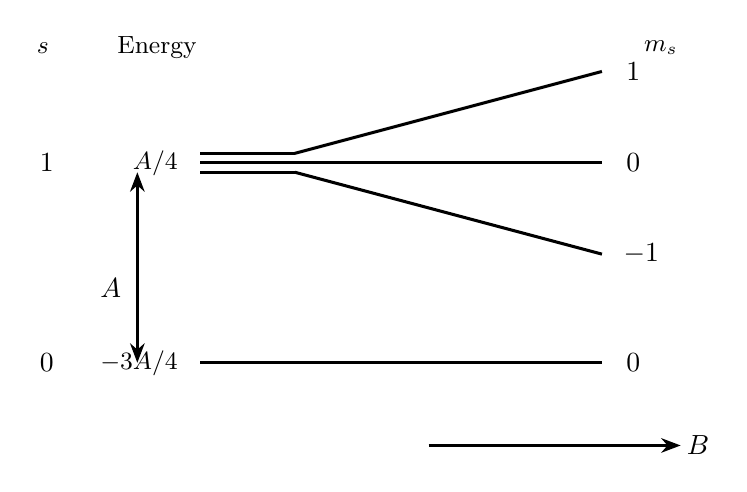
\begin{tikzpicture}[line width=1.1pt,>=Stealth]
% 表头
\node[font=\small] at (0.3,5.6) {$s$};
\node[font=\small] at (1.75,5.6) {Energy};
\node[font=\small] at (8.15,5.6) {$m_s$};
% 三重态（左侧靠拢的三条线，向右扇形展开）
\draw (2.3,4.02) -- (3.5,4.02);
\draw (2.3,4.14) -- (3.5,4.14);
\draw (2.3,4.26) -- (3.5,4.26);
\draw (3.5,4.26) -- (7.4,5.3);
\draw (3.5,4.14) -- (7.4,4.14);
\draw (3.5,4.02) -- (7.4,2.98);
% 单态
\draw (2.3,1.6) -- (7.4,1.6);
% 能量标注
\node[anchor=east,font=\small] at (2.15,4.14) {$A/4$};
\node[anchor=east,font=\small] at (2.15,1.6) {$-3A/4$};
% m_s 标记
\node at (7.8,5.3) {$1$};
\node at (7.8,4.14) {$0$};
\node at (7.9,2.98) {$-1$};
\node at (7.8,1.6) {$0$};
% s 标记
\node at (0.35,4.14) {$1$};
\node at (0.35,1.6) {$0$};
% 交换劈裂 A（双向箭头）
\draw[<->,line width=0.9pt] (1.5,1.6) -- (1.5,4.02);
\node[left=2pt] at (1.5,2.55) {$A$};
% 磁场 B 方向
\draw[->,line width=0.9pt] (5.2,0.55) -- (8.4,0.55);
\node at (8.62,0.55) {$B$};
\end{tikzpicture}
\end{document}
